%
%  PyMC User's Guide
%
%  Created by Chris Fonnesbeck on 2006-05-03.
%  Copyright (c) 2006 . All rights reserved.
%
\documentclass[]{book}

% Use utf-8 encoding for foreign characters
%\usepackage[utf8]{inputenc}

% Setup for fullpage use
\usepackage{fullpage}
\usepackage{amsmath}
\usepackage{epsfig}

% Flexible citation syntax
\usepackage{natbib}
% Uncomment some of the following if you use the features
%
% Running Headers and footers
%\usepackage{fancyheadings}

% Multipart figures
%\usepackage{subfigure}

% More symbols
%\usepackage{amsmath}
%\usepackage{amssymb}
%\usepackage{latexsym}

% Surround parts of graphics with box
\usepackage{boxedminipage}

% Package for including code in the document
\usepackage{listings}

% If you want to generate a toc for each chapter (use with book)
\usepackage{minitoc}

% This is now the recommended way for checking for PDFLaTeX:
\usepackage{ifpdf}

% Enable hyeprlinks
\usepackage[pdfpagemode=FullScreen,colorlinks=true,linkcolor=red]{hyperref}

%\newif\ifpdf
%\ifx\pdfoutput\undefined
%\pdffalse % we are not running PDFLaTeX
%\else
%\pdfoutput=1 % we are running PDFLaTeX
%\pdftrue
%\fi

\ifpdf
\usepackage[pdftex]{graphicx}
\else
\usepackage{graphicx}
\fi
\title{PyMC 2.0 svn User's Guide \\
Installation and tutorial}
\author{ Christopher Fonnesbeck\\ David Huard \\ Anand Patil }

% \date

% TODO: Logo.

\begin{document}

\ifpdf
\DeclareGraphicsExtensions{.pdf, .jpg, .tif}
\else
\DeclareGraphicsExtensions{.eps, .jpg}
\fi

\maketitle

\tableofcontents

\chapter{Introduction} %(fold)

Bayesian estimation, particularly using Markov chain Monte Carlo (MCMC), is an increasingly relevant approach to statistical estimation. However, few statistical software packages implement MCMC samplers, and they are non-trivial to code by hand. PyMC is a python module that implements the Metropolis-Hastings algorithm as a python class, and is extremely flexible and applicable to a large suite of problems. PyMC includes methods for summarizing output, plotting, goodness-of-fit and convergence diagnostics.

It is straightforward to code a simple MCMC sampler, using either the Gibbs or Metropolis-Hastings algorithm, in Python (or using a variety of other languages, for that matter). However, more complex models can be tricky to implement, each requiring its own unique sampler. A general, reusable sampler is desirable for use in applications, so that a new sampler need not be coded from scratch for every analysis. PyMC is a \href{http://python.org}{Python} module that provides a MCMC toolkit, making Bayesian simulation models relatively easy to implement.

\bigskip
PyMC is not an application per se. It consists of:
\begin{itemize}
    \item Two Python types, \texttt{Parameter} and \texttt{Node}, which are natural and extremely flexible building blocks for specifying arbitrary Bayesian statistical models.
    \item The \texttt{Model} class, which supervises MCMC loops and relieves users of the need for re-implementing utilities such as plotting, statistical summary, and recording samples in databases. This allows the user to concentrate on important aspects of the problem at hand, rather than the mundane details of statistical simulation.
    \item Fast, user-friendly and well-documented implementations of 24 common probability distributions.
    \item \textbf{XXX} Whatever we end up with with parallelization.
    \item The \texttt{SamplingMethod} class, which users can subclass to implement specialized algorithms on submodels. A handful of standard methods are included with the distribution.
\end{itemize}

PyMC aims to fully support newcomers to MCMC while providing the performance and flexibility statistical researchers need to develop new methods. As a Python package, it allows users to interface their MCMC algorithms with a wide range of other applications and analysis tools.

\section{How fast is PyMC?}\label{speed}
Python is a wonderful language, but it has an important drawback for statistical computing: like all interpreted languages, it's slow. PyMC aims to remedy this by implementing performance-critical portions in C, Fortran or NumPy. In basic usage, PyMC's speed is comparable to (whatever it's comparable to). Since there are several easy ways to write Python-callable C and Fortran modules, PyMC's speed can be greatly increased by writing application-optimized log-probability functions, which really isn't that hard.

Here are some speed results.

\section{Acknowledgments}\label{sec:acknowledgments}
The authors would like to thank the authors of PyMC's dependencies:
\begin{description}
	\item[numpy] \href{www.numpy.org/}{www.numpy.org/}
	\item[f2py] \href{cens.ioc.ee/projects/f2py2e/}{cens.ioc.ee/projects/f2py2e/}
	\item[matplotlib] \href{matplotlib.sourceforge.net/}{matplotlib.sourceforge.net/}
	\item[ipython1] \href{ipython.scipy.org/moin/IPython1}{ipython.scipy.org/moin/IPython1}
	\item[pydot] \href{dkbza.org/pydot.html}{dkbza.org/pydot.html}
	\item[epydoc] \href{epydoc.sourceforge.net/}{epydoc.sourceforge.net/}
	\item[pytables] \href{www.pytables.org/}{www.pytables.org/}					
	\item[pysqlite] \href{?}{?}					
\end{description}

And of course Python, \href{www.python.org/}{www.python.org/}.

%(end)

\chapter{Installation} %(fold)

PyMC is known to run on Mac OS X, Linux and Windows, but in theory should be able to work on just about any platform for which Python is available (and there are many). Rather than a standalone application, PyMC is simply a \emph{module} for the Python programming language. That is, a set of programming classes that are imported into the Python programming environment for subsequent use. The classes are very general, and can therefore be implemented in a variety of Bayesian analytic tasks. I will describe how to install PyMC using both binary installers (for Mac and Windows) and builds from source code.

Pre-built binary and source distributions of PyMC are available from \href{http://trichech.us}{trichech.us}. There are three PyMC distribution formats provided, each containing the same PyMC module, but targeted for different computing platforms. For Macintosh (OS X) users there is an installer package (.mpkg), for Linux users a compressed tar (.tar.gz) source archive, and for Microsoft Windows a binary executable installer (note that this may not always be the latest version, as PyMC is not specifically developed or tested for Windows).

PyMC requires some prerequisite packages to be present on the system before the PyMC package itself is installed. Fortunately, there are currently only a few dependencies, and all are freely available online.
\begin{itemize}

\item Python version 2.4 or later. I recommend using the \href{http://www.activestate.com/Products/ActivePython/}{ActiveState distributions} for Mac OS X and Linux. Windows users should download and install \href{http://code.enthought.com/enthon/}{Enthought Python}, which contains all of the required packages below. Additionally, the Mac OS X binary distribution of PyMC comes bundled with these prerequisites.

\item FORTRAN and C compilers, preferably G77 and GCC (\emph{i.e.} the GNU compilers), respectively. You may use other compilers, but most have not been tested with PyMC.

\item \href{http://numeric.scipy.org/}{Numpy}, latest version. This is a fundamental scientific programming package for python, which replaces a slew of stand-alone packages (including Numeric) that needed to be installed in the past.

\item \href{http://matplotlib.sourceforge.net/}{Matplotlib} version 0.86 or later. This package is used for plotting of MCMC output.
\end{itemize}


\section{Platform-specific instructions}
\subsection{Mac OS X}

If you double-click the installer package, your archive utility will usually expand the installer from its archive. From here, the prerequisite packages can be installed (by double-clicking the installers and following the on-screen instructions), followed by the PyMC package itself.

If you wish to build and install PyMC from source, first ensure that you are using GCC 3.3 (on newer OS X systems GCC 4.0.1 is the default):
\begin{verbatim}
sudo gcc_select 3.3
\end{verbatim}
Then, untar the source archive, then move into the resulting source directory in the command terminal and type:
\begin{verbatim}
python setup.py build
sudo python setup.py install
\end{verbatim}
The \verb=sudo= command is required to install PyMC into the Python site-packages directory, which should have restricted privileges. You will be prompted for a password, and provided you have superuser privileges, the installation will proceed.

\subsection{Linux}

Unfortunately, binary installers are not currently available for Linux systems, but it is straightforward to build the package yourself. Simply untar the package archive, then move to the resulting archive directory and type:
\begin{verbatim}
python setup.py build
sudo python setup.py install
\end{verbatim}

\subsection{Windows}

Simply double-click the executable installation package, and follow the on-screen instructions.
If you wish to build and install PyMC from source, untar the source archive, then move into the resulting source directory in the command terminal and type:
\begin{verbatim}
python setup.py build --compiler=mingw32 install
\end{verbatim}
This assumes you are using the GCC compiler (recommended). Otherwise, change the --compiler argument accordingly.

\section{Testing the Installation}

If there were no errors in the installation process, it was probably successful. Start python and try importing PyMC\footnote{If you are running from the command line, you may have to move to another directory before running python and importing the PyMC module; for example, switch to your home directory: \textbf{cd \textasciitilde}}
\begin{verbatim}
>>> import PyMC
\end{verbatim}
Once the module has been imported, try running the test:
\begin{verbatim}
>>> PyMC.unittest.main()
\end{verbatim}

This test model estimates the switch point between two rate distributions within a time series of coal mining disasters in the UK. If successful, the test should run two chains for 10000 iterations each, then produce some output. Provided that the test runs without incident, you are now ready to start working with PyMC. The remainder of this document deals with building MCMC models in PyMC. I will touch on some essential theory, but will assume a working knowledge of both basic statistical probability and the Python programming language. If you require an introduction to Python, or a refresher, I recommend the online guide \href{http://www.ibiblio.org/obp/thinkCSpy/index.htm}{``How to Think Like a Computer Scientist: Learning with Python"}. Additionally, there are a number of \href{http://rgruet.free.fr/PQR24/PQR2.4.html}{quick reference} pages available online that summarize most of the common Python syntax. For those who require more statistical preparation, a freely-distributable (GNU public license) text \href{https://www.dartmouth.edu/~chance/teaching_aids/books_articles/probability_book/amsbook.mac.pdf}{``Introduction to Probability''} is available for download in PDF format.

%(end)
\chapter{Model building in PyMC} %(fold)

\section{Bayesian statistical models}
We assume that the reader has at least some familiarity with probability and Bayesian statistics. If you don't understand the notation in this section, please consult \citet{Gelman:1996gp}.

Bayesian statistical inference begins with specification of a probability model relating inferential targets to data. For example, consider the following dataset, which is a time series of recorded coal mining disasters in the UK from 1851 to 1962.
\begin{center}
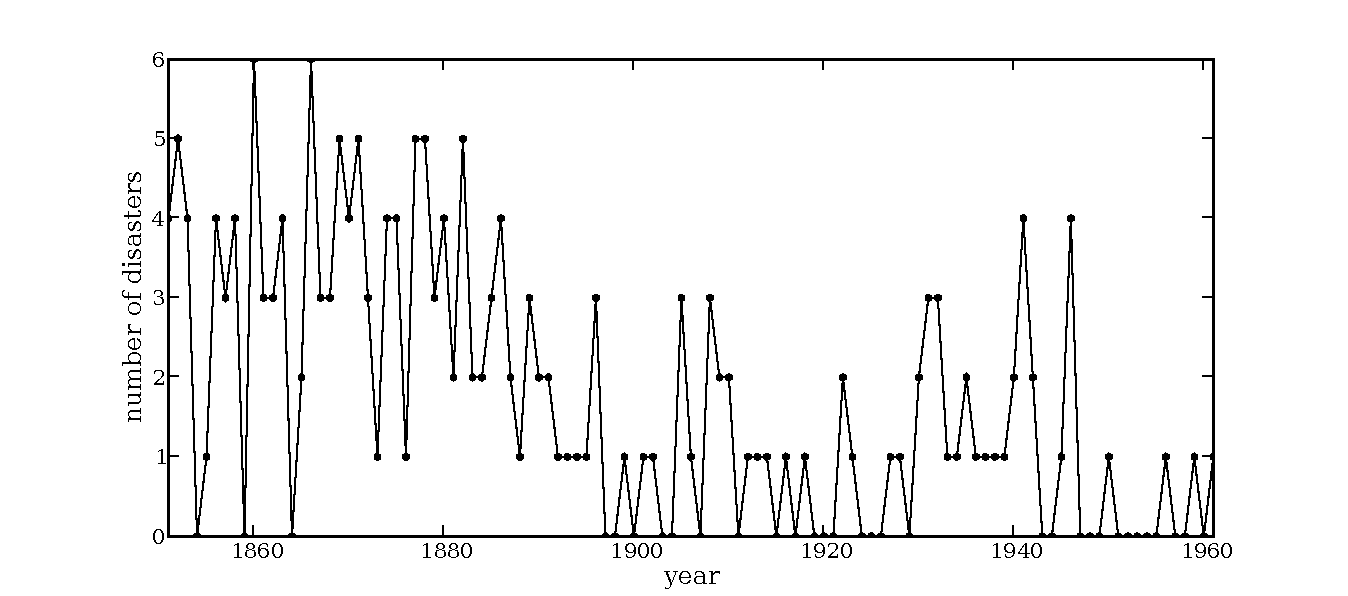
\epsfig{file=disaster_ts.pdf, width=15cm}
\end{center}
Occurrences of disasters in the time series is thought to be derived from a Poisson process with a large rate parameter in the early part of the time series, and from one with a smaller rate in the later part. We are interested in locating the change point in the series, which perhaps is related to changes in mining safety regulations.

We represent our conceptual model formally as a statistical model:
\begin{eqnarray*}
(D_t | s, e, l) \sim \textup{Po}\left(r_t\right), & r_t=\left\{\begin{array}{ll}
    e & t\le s\\ l & t>s
    \end{array}\right.,&t\in[1851,1962]\\
s\sim \textup{U}(1851, 1962)\\
e\sim \textup{Exp}(1)\\
l\sim \textup{Exp}(1)
\end{eqnarray*}
The symbols have the following meanings:
\begin{description}
    \item[$D_t$:] The number of disasters in year $t$.
    \item[$r_t$:] The rate parameter of the Poisson distribution of disasters in year $t$.
    \item[$s$:] The year in which the rate parameter changes.
    \item[$e$:] The rate parameter before the switchpoint $s$.
    \item[$l$:] The rate parameter after the switchpoint.
\end{description}

The product
\begin{eqnarray*}
\prod_t p(D_t|s,e,l) p(s)p(e)p(l)
\end{eqnarray*}
gives the joint distribution $p(D,s,e,l)$ of the data and unknown parameters. This is proportional to the posterior distribution $p(s,e,l|D)$ (where $D$ collects $D_t$ for $t$ from 1851 to 1962).

In the term $p(D_t|s,e,l)$, $D_t$ is called the \emph{consequent} and $s$, $e$ and $l$ are called the \emph{antecedents}. The antecedents are sometimes called the \emph{parents} of a consequent, and the set of variables that claim a particular variable as a parent are called that variables \emph{children}. This terminology is used in PyMC.

The dependence structure of a statistical model can be represented by a \emph{directed acyclic graph}. For our coal-mining disaster model, the PyMC-generated DAG is illustrated in figure \ref{fig:disaster_dag}. The arrows in the figure point from parent to child, or alternatively from antecedent to consequent.

\begin{figure}[hhhhhhhhhhh]
\begin{center}
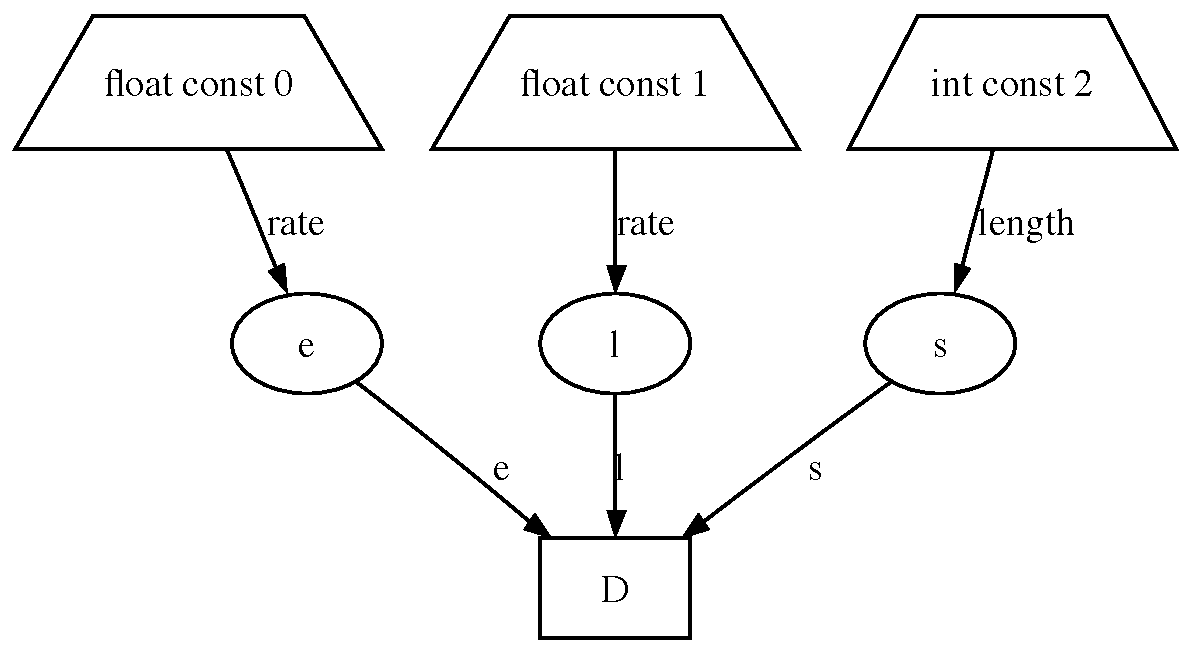
\epsfig{file=DisasterModel.pdf,width=7cm}
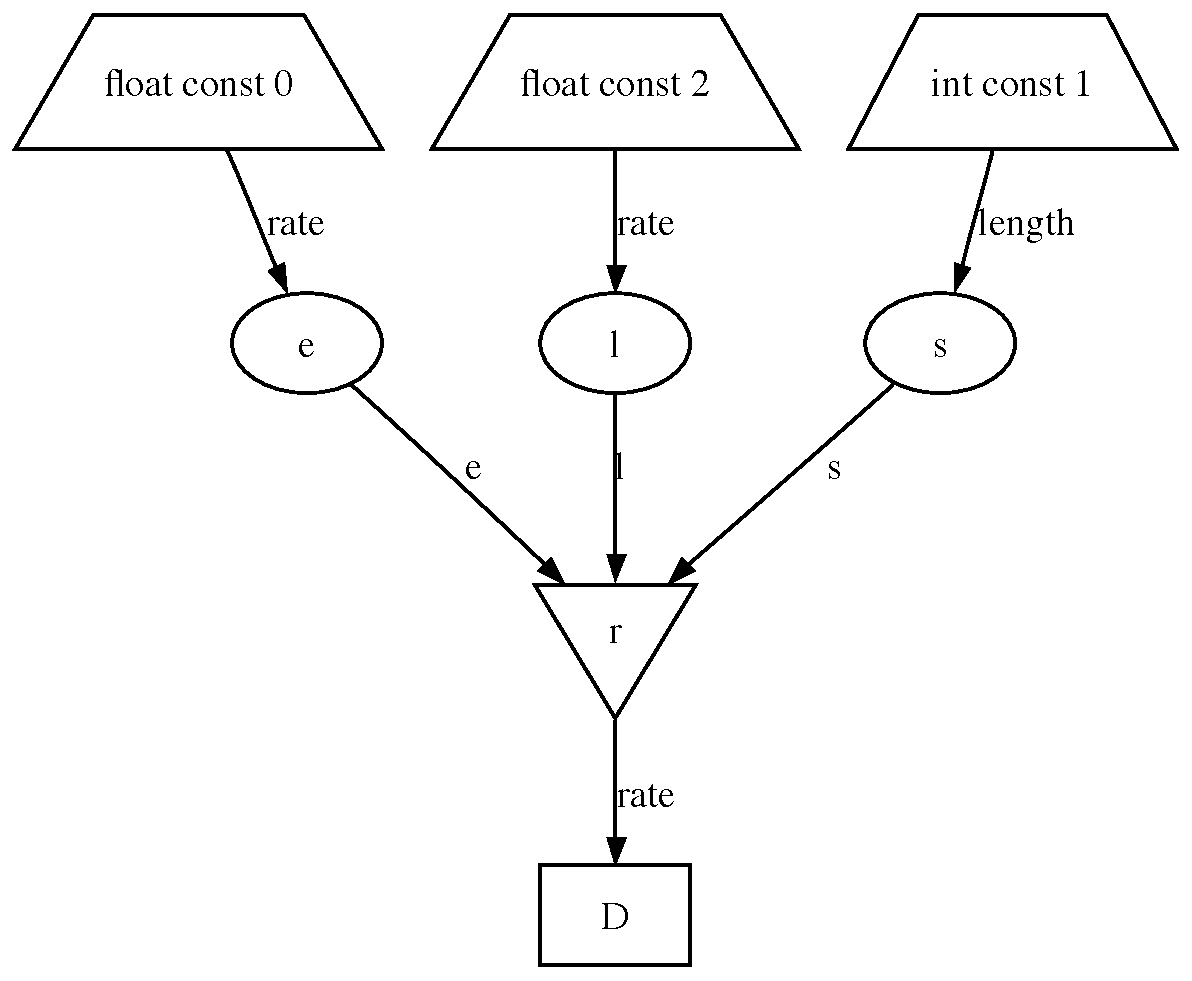
\epsfig{file=DisasterModel2.pdf,width=7cm}
\caption{\textbf{Left:} A DAG of the coal-mining disaster example with the function $r_t$ implicit. \textbf{Right:} An equivalent DAG with $r_t$ explicit. The `float const's refer to the parameters of the priors of $e$, $l$ and $s$. The labels on the arrows refer to the parameter names assigned to the parents by the child. For example, in the DAG on the right $D$ considers $r$ to be its `rate' parameter.
}
\label{fig:disaster_dag}
\end{center}
\end{figure}

In principle, we could have written down other statistical models that gave the same joint distribution (and hence the same posterior distribution). For example, we could have specified the model as
\begin{eqnarray*}
p(s|D,l,e)\prod_tp(D_t|l,e,D_{1851\ldots t-1})p(l)p(e),
\end{eqnarray*}
and drawn a new DAG representation of the dependence structure. However, that would have been extremely uncomfortable. Our intuition tells us that $e$, $l$ and $s$ influence $D_t$, not that $D_t$, $e$ and $l$ influence $s$. In other words, the statement
\begin{quote}
Given the rate parameter before the switchpoint, the rate parameter after the switchpoint, and the switchpoint itself, the distribution of disasters in year $t$ is $d$.
\end{quote}
is much more natural than the statement
\begin{quote}
Given the rate parameter befare the switchpoint, the rate parameter after the switchpoint, and annual disasters up to year $t-1$, the distribution of disasters in year $t$ is $d^*$. Further, given all the data on annual disasters the distribution of the switchpoint is $d^{**}$.
\end{quote}

Bayesian methods, and statistics in general, are usually needed \emph{because} it's natural to think of the data as consequences of the inferential targets. This point can be counterintuitive at first, as most scientists' instinct is to regard data as fixed a priori and unknown parameters' values as dependent on the data. However, it's important to understand for effective model-building in PyMC.



\section{\texttt{Parameter} and \texttt{Node}}\label{sec:PyMCObjects}
PyMC provides two built-in types to serve as the building blocks of Bayesian probability models in Python. A parameter object represents a variable whose distribution depends on its parents, but which is not completely determined by its parents. This is sometimes referred to as a random variable, though it need not be random in the frequentist sense. In the coal-mining disaster model, $s$, $l$, $e$ and $D$ are all parameters, but $r$ is not. Since the value of $D$ has been observed, its \texttt{isdata} flag would be set to true; see section \ref{sub:@data}. A node object, on the other hand, represents a variable that is completely determined by its parents. In the coal-mining disaster model, $r$ is a node.

These objects are meant to do only what their mathematical counterparts `do,' and to do it efficiently. As such, they have very limited awareness of the probability model in which they are embedded and no methods for updating their values in an MCMC loop given the rest of the model. PyMC leaves parameter updating functionality to the \texttt{SamplingMethod} class (sec \ref{sec:SamplingMethod}) and model-level functionality to the \texttt{Model} class (sec \ref{sec:Model})

PyMC also provides a special container class for parameters and nodes to ease programming of certain dependency situations, such as when a particular variable depends on every element of a Markov chain.

\subsection{\texttt{Parameter}}\label{sub:parameter}

Parameters expose the following attributes:
\begin{description}
    \item[\texttt{parents}:] A dictionary containing self's parents. The keys of the dictionary correspond to the names assigned to self's parents by self, and the values correspond to the actual parents. For example, a normally-distributed parameter's parents would probably be keyed as \texttt{mu} and \texttt{tau}, \texttt{V} or \texttt{sigma}. Since PyMC inherits Python's weak typing, parents may be of any class or type.
    \item[\texttt{children}:] A set containing self's children, which must be parameters or nodes. This set is produced automatically; the user doesn't need to worry about filling it.
    \item[\texttt{value}:] Self's current value, which is updated many times over the course of an MCMC loop. Attempts to update this attribute raise an error if \texttt{isdata} is true. Again, this may be of any class or type.
    \item[\texttt{isdata}:] A boolean indicating whether the self's value has been observed (is fixed).
    \item[\texttt{trace}:] The trace object assigned to self, see \textbf{XXX}.
    \item[\texttt{logp}:] The log-probability or log-density of self's current value, conditional on self's parents' current values. This attribute is automatically updated every time it is accessed. In addition, \texttt{Parameter} caches its most recent log-probabilities to avoid unnecessary recomputation. See section \ref{sub:caching}.
    \item[\texttt{\_\_name\_\_}:] The name of the parameter, should be unique.
    \item[\texttt{\_\_doc\_\_}:] The docstring of the parameter.
\end{description}

Parameters have the following methods:
\begin{description}
	\item[\texttt{touch()}:] PyMC parameters and nodes cache the last few values of their arguments. If a parameter's log-probability or a node's value is queried when their arguments' value configuration is in their cache, they don't recompute. This is called `memoization'. The price of this optimization is that parameters' values can't be updated in-place, or else the next recompute may be incorrectly skipped. If you update a parameter's value in-place, be sure to call this method afterward. It simply replaces the parameter's value with a shallow copy of itself.
    \item[\texttt{random()}:] This causes self to draw its value from its distribution conditional on its parents, and returns that value. This is useful for model averaging and certain Metropolis-Hastings algorithms. Raises an error if no \texttt{random} argument was passed to the constructor (ie, if the `medium' interface was used, see below).
\end{description}

\subsubsection{Instantiation}
In order to make specification of standard probability models easy while making room for specification of even the most exotic probability model, PyMC provides four ways to instantiate parameters.
\begin{description}
    \item[Short] \textbf{XXX}
    \item[Medium] A normally-distributed parameter called \texttt{A} could be instantiated using the medium interface as follows:
    \begin{verbatim}
@parameter
def A(value=3., mu=B, tau=C):
    """Parameter A is normally distributed."""
    return 0.5 * tau * (value-mu)**2 + 0.5*log(0.5*tau/PI)
    \end{verbatim}
    The decorator \texttt{parameter} turns the function \texttt{A} into a parameter which evaluates its log-probability using \texttt{A}. The \texttt{value} argument, which is required, provides an initial value for the parameter. The names of the function's other arguments become the keys of the parameter's \texttt{parents} dictionary, which maps to the corresponding values (parent objects). The name of the function (in this case \texttt{A}) becomes the \texttt{\_\_name\_\_} of the parameter, and the docstring of the function is passed on to the parameter as well.

    The parameter may be valued as any object, its parents may be any objects, and there is absolutely no restriction on the log-probability function, as long as it returns a \texttt{float}. Note that, although the log-probability function is written out for illustration, it would be much faster to return \texttt{normal\_like(value, mu, tau)}

    The medium interface's decorator can take a flag called \texttt{trace} which signals to \texttt{Model} whether an MCMC trace should be kept for this parameter: \texttt{@parameter(trace = False)}.
    \item[Long] The long interface extends the medium interface by allowing the user to specify a method for sampling the parameter's value conditional only on its parents.
    \begin{verbatim}
@parameter
def A(value=3., mu=B, tau=C):
    """Parameter A is normally distributed."""

    def logp(value, mu, tau):
        return 0.5 * tau * (value-mu)**2 + 0.5*log(0.5*tau/PI)

    def random(mu, tau):
        return rnormal(mu, tau)

    rseed = 1.
    \end{verbatim}
The parameter again gets its name, docstring and parents from \texttt{A}, but in this case it will evaluate its log-probability using the \texttt{logp} function. The \texttt{random} function is used when \texttt{Parameter.random()} is called. Note that it doesn't take a \texttt{value} argument, because it provides a new value. \textbf{XXX} \texttt{rseed} provides a seed for the RNG.

    \item[Direct] Some users may prefer not to use the \texttt{parameter} decorator, but to instantiate \texttt{Parameter} directly:
\begin{verbatim}
def A_logp(value, mu, tau):
    return 0.5 * tau * (value-mu)**2 + 0.5*log(0.5*tau/PI)

A = Parameter(logp = A_logp, name = 'A', value = 3.,
parents = {'mu': B, 'tau': C}[,
doc = 'Parameter A is normally distributed',
random = rnormal, trace = True, rseed = 1., isdata = False,
cache_depth = 2])
\end{verbatim}
\end{description}



\subsection{The \texttt{data} decorator}\label{sub:@data}
In the medium and long interfaces, the parameter's \texttt{isdata} flag can be set to true by replacing \texttt{@parameter} with \texttt{@data}.


\subsection{\texttt{Node}}\label{sub:node}

Nodes expose the following attributes:
\begin{description}
    \item[\texttt{parents}:] A dictionary containing self's parents. The keys of the dictionary correspond to the names assigned to self's parents by self, and the values correspond to the actual parents. Since PyMC inherits Python's weak typing, parents may be of any class or type.
    \item[\texttt{children}:] A set containing self's children, which must be parameters or nodes. This set is produced automatically; the user doesn't need to worry about filling it.
    \item[\texttt{value}:] Self's current value. Unlike parameter, self's value depends on its parents. As with parameter's \texttt{logp} attribute, this attribute is automatically updated every time it is accessed. Nodes cache their last few values to avoid unnecessary recomputation. Attempts to update this attribute raise an error.
    \item[\texttt{trace}:] The trace object assigned to self, see \textbf{XXX}.
    \item[\texttt{\_\_name\_\_}:] The name of the node, should be unique.
    \item[\texttt{\_\_doc\_\_}:] The docstring of the node.
\end{description}
Nodes have no methods.

\subsubsection{Instantiation}
Nodes are less complicated than parameters, and PyMC provides only two ways to instantiate them:
\begin{description}
    \item[Decorator] A node can be instantiated via a decorator in a way very similar to parameter's medium interface:
\begin{verbatim}
@node
def D(arg_1 = E, arg_2 = F)
    """The D node"""
    return sqrt(arg_1 ** 2 + arg_2 ** 2)
\end{verbatim}
The function supplied should return a new value for the node (which, again, may be any object). Arguments' keys and values are converted into a parent dictionary as with parameter's medium interface. The function's \texttt{\_\_name\_\_} is passed on to the node.
    \item[Direct] The same node could be instantiated directly as follows:
\begin{verbatim}
def D_eval(arg_1, arg_2):
    return sqrt(arg_1 ** 2 + arg_2 ** 2)

D = Node(eval = D_eval, name = 'D',
parents = \{'arg_1': E, 'arg_2': F\})[],
doc = 'The D node',
trace = True),
cache_depth = 2]
\end{verbatim}
The \texttt{trace} flag signals to \texttt{Model} whether to keep a trace for self, as with parameter.
\end{description}
Note that nodes have no \texttt{isdata} flag. If a node's value were known, its parents would be restricted to the inverse image of that value under the node's evaluation function. This usage case would be extremely difficult to support in generality, but it can be implemented for particular applications at the \texttt{SamplingMethod} level.

\subsection{The \texttt{PyMCObjectContainer} class for arrays of parameters and nodes}\label{sub:container}
In the following hypothetical situation, it would be inconvenient to assign a unique label to each parent of $B$:
\begin{eqnarray*}
	A_0 \sim \textup N(0,V)\\
	A_{i+1}|A_i\sim\textup{N(0,V)},&i=1\ldots N\\
	B \sim \textup N\left(\sum_{i=0}^N A_i,W\right).
\end{eqnarray*}

This situation can be handled using the \texttt{PyMCObjectContainer} class as follows:
\begin{verbatim}
@parameter
def A(value=0., mu=0., V=V):
    """The initial value"""
    return normal_like(value, mu, V)
Alist = [A]

for i in range(1,N):
    @parameter
    def A(value=0., mu=Alist[i-1], V=V):
        """value %i""" % i
        return normal_like(value, mu, V)
    Alist.append(A)
    
A = PyMCObjectContainer(A)

@data
def B(value=0., mu=A, V=W):
    """The sum of the Markov chain"""
    return normal_like(value, sum(mu), V)   
\end{verbatim}
This works because PyMC object containers, like parameters and nodes, expose an attribute called \texttt{value}. This attribute returns a copy of the (possibly nested) iterable that was passed into the container at instantiation, but with each instance of a parameter or node replaced with \emph{its} value. Note that simply writing
\begin{verbatim}
@data
def B(value=0., mu=Alist, V=W):
	"""The sum of the Markov chain"""
	return normal_like(value, sum(mu), V)	
\end{verbatim}
would not have worked, because \texttt{list} does not expose an attribute called \texttt{value}. PyMC object containers can currently be constructed from any object that has a \texttt{\_\_getitem\_\_} method (such as lists, tuples, and numpy arrays), but not from sets.

\subsection{Examples}\label{sub:example}
Here is the coal-mining disaster model implemented in PyMC with $r$ implicit, as in the left pane of figure \ref{fig:disaster_dag}:
\begin{verbatim}
@parameter
def s(value=50, length=110):
    """Change time for rate parameter."""
    constrain(value, 0, length)
    return 0.

@parameter
def e(value=1., rate=1.):
    """Rate parameter of poisson distribution."""
    return exponential_like(value, rate)

@parameter
def l(value=.1, rate = 1.):
    """Rate parameter of poisson distribution."""
    return exponential_like(value, rate)

@data
def D(  value = D_array,
        switchpoint = s,
        early_mean = e,
        late_mean = l):
    """Annual occurences of coal mining disasters."""
    return poisson_like(value[:s],e) + poisson_like(value[s:],l)
\end{verbatim}
To make $r$ explicit as in the right pane of figure \ref{fig:disaster_dag}, we would write:
\begin{verbatim}
@parameter
def s(value=50, length=110):
    """Change time for rate parameter."""
    constrain(value, 0, length)
    return 0.

@parameter
def e(value=1., rate=1.):
    """Rate parameter of poisson distribution."""
    return exponential_like(value, rate)

@parameter
def l(value=.1, rate = 1.):
    """Rate parameter of poisson distribution."""
    return exponential_like(value, rate)

@node
def r(l=l,e=e,s=s):
    """r = function(l,e,s)"""
    ret_val =  ones(111,dtype=float)
    ret_val[:s] = e
    ret_val[s:] = l
    return ret_val

@data
def D(  value = D_array, rate=r):
    """Annual occurences of coal mining D."""
    return poisson_like(value,rate)
\end{verbatim}
In general, it's better to make heavyweight functions into their own nodes, because nodes' caches avoid unnecessary recomputation. In this case, however, the version with $r$ implicit is quite a bit faster.

\section{The \texttt{Model} class} \label{sec:Model} 
This class serves as a container for probability models and as a stem class for other `model-level' classes like \texttt{Sampler}. Methods implemented:
\begin{description}
	\item[\texttt{sample\_model\_likelihood()}:] Returns an estimate of $\log p(d|M)$, the unconditional log-probability or log-density of all the data objects in model $M$. This is called by the function \texttt{weight()}, which finds the posterior probabilities of a set of models.
	\item[\texttt{DAG()}:] Outputs a graphical representation of the model.
	\item[\texttt{tally()}:] Tells all parameters and nodes to record their current values in their traces.
	\item[\texttt{remember()}:] Tells all parameters and nodes to set their values to a certain element of their traces.
	\item[\texttt{save\_state()}:] Under construction.
	\item[\texttt{save\_traces()}:] Under construction.
	\item[\texttt{seed()}:] All parameters with an \texttt{rseed} value draw a new value from their distributions.
\end{description}

Useful attributes:
\begin{description}
	\item[\texttt{containers}:] A set of self's PyMC object containers.
	\item[\texttt{parameters}:] A set of self's parameters.
	\item[\texttt{nodes}:] A set of self's nodes.
	\item[\texttt{data}:] A set of self's data objects.
\end{description}

\chapter{Model fitting with PyMC} %(fold)
\label{chap:MCMC}

%MCMC methods are algorithms that sample from probability distributions (\emph{i.e.} Monte Carlo simulation) to yield Markov chains.

\section{Monte Carlo Methods in Bayesian Analysis}

Bayesian model specification often results in posterior forms that are difficult to manipulate analytically. Expand- when data are children of other parameters, it's not natural to simulate directly. However, it is often possible to generate simulated values that share the distributional properties of the specified posterior. Such simulations may be summarized in such a way that describes the posterior density. For example, consider the expected value of some integral quantity:

\[
E[{\bf x}] = \int_{-\infty}^{\infty} {\bf x} f({\bf x}) d{\bf x}, \qquad
{\bf x} = \{x_1,...,x_k\}
\]

\noindent where $k$ is perhaps very large, making the joint distribution of ${\bf x}$ analytically complex. If we can produce random vectors $\{{\bf x_i}\}$, we can use these values to approximate the unknown integral. This process is known as {\emph Monte Carlo integration}. In general, MC integration says that:

\[
I[a,b] = \int_a^b h(x) f(x) dx
\]

\noindent can be estimated by:

\[
\hat{I}[a,b] = \frac{1}{n}\sum_{i=1}^n h(x_i)
\]

\noindent This estimate is useful because:

\begin{itemize}
\item
By the strong law of large numbers:
\[\hat{I}[a,b] \rightarrow I[a,b] \mbox{with probability 1}\]
\item
Simulation error can be measured and controlled:
\[Var(\hat{I}[a,b]) = \frac{1}{n(n-1)}\sum_{i=1}^n (h(x_i)-\hat{I}[a,b])^2\]
\end{itemize}

Why is this relevant to Bayesian analysis? If we replace $f(x)$ with a posterior, $\pi(\theta|x)$ and make $h(x)$ an interesting function of the unknown parameter, the resulting expectation is that of the posterior of $h(\theta)$:

\[
E[h(\theta|x)] = \int \pi(\theta|x) h(\theta) d\theta \approx \frac{1}{n}\sum_{i=1}^n h(\theta)
\]

\subsection{Rejection Sampling}

Though Monte Carlo integration allows us to estimate integrals that are unassailable by analysis, it relies on the ability to draw samples from the posterior distribution. For known parametric forms, this is not a problem; probability integral transforms or bivariate techniques (e.g Box-Muller method) may be used to obtain samples from uniform pseudo-random variates generated from a computer. Often, however, we cannot readily generate random values from non-standard posteriors. In such instances, we can use rejection sampling to generate samples.

\begin{figure}[ht]
        \begin{center}
        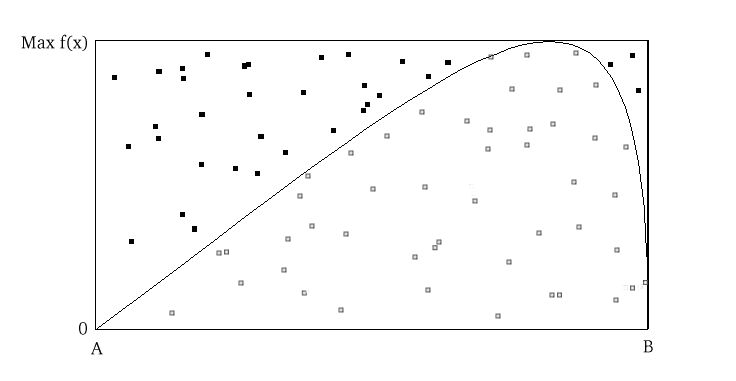
\includegraphics[scale=0.4]{reject.png}
    \end{center}
    \caption{Rejection sampling of a bounded form. Area is estimated by the ratio of accepted (open squares) to total points, multiplied by the rectangle area.}
    \label{fig:bound}
\end{figure}

Posit a function, $f(x)$ which can be evaluated for any value on the support of $x:S_x = [A,B]$, but may not be integrable or easily sampled from. If we can calculate the maximum  value of $f(x)$, we can then define a rectangle that is guaranteed to contain all possible values $(x,f(x))$. It is then trivial to generate points over the box and enumerate the values that fall under the curve (Figure \ref{fig:bound}).

\[
\frac{\mbox{Points under curve}}{\mbox{Points generated}} \times \mbox{box area} = \lim_{n \to \infty} \int_A^B f(x) dx
\]

\begin{figure}[h]
        \begin{center}
        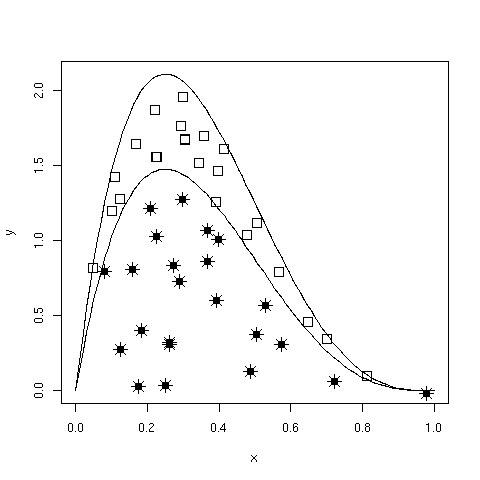
\includegraphics[scale=0.4]{envelope.png}
    \end{center}
    \caption{Rejection sampling of an unbounded form using an enveloping distribution.}
    \label{fig:unbound}
\end{figure}

\noindent This approach is useful, for example, in estimating the normalizing constant for posterior distributions.

If $f(x)$ has unbounded support (i.e. infinite tails), such as a Gaussian distribution, a bounding box is no longer appropriate. We must specify a majorizing (or, enveloping) function, $g(x)$, which implies:

\[
g(x) \le  f(x) \qquad\forall x \in (-\infty,\infty)
\]

Having done this, we can now sample ${x_i}$ from $g(x)$ and accept or reject each of these values based upon $f(x_i)$. Specifically, for each draw $x_i$, we also draw a uniform random variate $u_i$ and accept $x_i$ if $u_i < f(x_i)/kg(x_i)$ (Figure \ref{fig:unbound}). This approach is made more efficient by choosing an enveloping distribution that is ``close'' to the target distribution, thus maximizing the number of accepted points. Further improvement is gained by using optimized algorithms such as importance sampling (see text) which, as the name implies, samples more frequently from important areas of the distribution.

\section{Markov Chains}

A Markov chain is a special type of \emph{stochastic process}. The standard definition of a stochastic process is an ordered collection of random variables:

\[
\{X_t:t \in T\}
\]

\noindent where $t$ is frequently (but not necessarily) a time index. If we think of $X_t$ as a state $X$ at time $t$, and invoke the following dependence condition on each state:

\[
Pr(X_{t+1}=x_{t+1} | X_t=x_t, X_{t-1}=x_{t-1},\ldots,X_0=x_0) = Pr(X_{t+1}=x_{t+1} | X_t=x_t)
\]

\noindent then the stochastic process is known as a Markov chain. This conditioning specifies that the future depends on the current state, but not past states. Thus, the Markov chain wanders about the state space, remembering only where it has just been in the last time step. The collection of transition probabilities is sometimes called a \emph{transition matrix} when dealing with discrete states, or more generally, a \emph{transition kernel}. In the context of Markov chain Monte Carlo, useful to think of the Markovian property as ``mild non-independence''\footnote{In general, for Bayesian analyses, statistical independence is less relevant, relative to classical statistical inference. Instead, we substitute the notion of \emph{exchangeability}, which is a weaker concept, but often just as useful. Exchangeability essentially implies that different permutations (orderings) of a sequence of random variables will have the same marginal distribution. A sequence of random quantities may not be considered independent in a Bayesian sense, but are frequently exchangeable.}. We will see that, while it may be difficult to generate independent samples from a particular posterior distribution, it may be possible to generate dependent samples that may be useful in describing that distribution.

\subsection{Jargon-busting}

Before we move on, it is important to define some general properties of Markov chains. They are frequently encountered in the MCMC literature, and some will help us decide whether MCMC is producing a useful sample from the posterior.

\begin{itemize}
\item \emph{Homogeneity}: A Markov chain is homogeneous at step $t$ if the transition probabilities are independent of the state at $t$. The starting point of the chain is almost never homogeneous, as the initial values are either hand-picked or arbitrary.
\item \emph{Irreducibility}: A Markov chain is irreducible if every state is accessible in one or more steps from any other state. That is, the chain contains no absorbing states. This implies that there is a non-zero probability of eventually reaching state $k$ from any other state in the chain.
\item \emph{Recurrence}: States which are visited repeatedly are \emph{recurrent}. If the expected time to return to a particular state is bounded, this is known as \emph{positive recurrence}, otherwise the recurrent state is \emph{null recurrent}. Further, a chain is \emph{Harris recurrent} when it visits all states $X \in S$ infinitely often in the limit as $t \to \infty$; this is an important characteristic when dealing with unbounded, continuous state spaces. Whenever a chain ends up in a closed, irreducible set of Harris recurrent states, it stays there forever and visits every state with probability one.
\item \emph{Stationarity}: A stationary Markov chain produces the same marginal distribution when multiplied by the transition kernel.  Thus, if $P$ is some $n \times n$ transition matrix:

\[{\bf \pi P} = {\bf \pi}\]

\noindent for Markov chain $\pi$. Thus, $\pi$ is no longer subscripted, and is referred to as the \emph{limiting distribution} of the chain. In MCMC, the chain explores the state space according to its limiting marginal distribution.
\item \emph{Ergodicity}: Ergodicity is an emergent property of Markov chains which are irreducible, positive Harris recurrent and aperiodic. Ergodicity is defined as:

\[
\lim_{n \to \infty} Pr^{(n)}(\theta_i,\theta_j) = \pi(\theta_j) \quad \forall \theta_i, \theta_j \in \Theta
\]

\noindent or in words, the marginal distribution of the chain is the same at one step as at all other steps. This implies that our Markov chain, which we recall is dependent, now generates quantities that are independent. If it means anything to you, ergodicity is the analogue of the strong law of large numbers for Markov chains. For example, take values $\theta_{i+1},\ldots,\theta_{i+n}$ from a chain that has reached an ergodic state. A statistic of interest can then be estimated by:

\[
\hat{h}(\theta) = \frac{1}{n}\sum_{j=i+1}^{i+n} h(\theta_j) \approx h(\theta)
\]

\end{itemize}

\section{Why MCMC Works: Reversible Markov Chains}

Markov chain Monte Carlo simulates a Markov chain for which some function of interest (\emph{e.g.} the joint distribution of the parameters of some model) is the unique, invariant limiting distribution. An invariant distribution with respect to some Markov chain with transition kernel $Pr(y \mid x)$ implies that:
\[
\int_x Pr(y \mid x) \pi(x) dx = \pi(y),
\]
and similarly:
\[
\int_y Pr(x \mid y) \pi(y) dy = \pi(x),
\]

Invariance is guaranteed for any \textbf{reversible} Markov chain. Consider a Markov chain in reverse sequence: $\{\theta^{(n)},\theta^{(n-1)},...,\theta^{(0)}\}$. This sequence is still Markovian, because:
\[
Pr(\theta^{(k)}=y \mid \theta^{(k+1)}=x,\theta^{(k+2)}=x_1,\ldots ) = Pr(\theta^{(k)}=y \mid \theta^{(k+1)}=x)
\]
Forward and reverse transition probabilities may be related through Bayes theorem:
\begin{eqnarray}
Pr(\theta^{(k)}=y \mid \theta^{(k+1)}=x) &=& \frac{Pr(\theta^{(k+1)}=x \mid \theta^{(k)}=y) Pr(\theta^{(k)}=y)}{Pr(\theta^{(k+1)}=x)} \nonumber \\
&=& \frac{Pr(\theta^{(k+1)}=x \mid \theta^{(k)}=y) \pi^{(k)}(y)}{\pi^{(k+1)}(x)} \nonumber
\end{eqnarray}

\[
\frac{Pr(\theta^{(k+1)}=x \mid \theta^{(k)}=y) \pi^{(k)}(y)}{\pi^{(k+1)}(x)}
\]

\noindent Though not homogeneous in general, $\pi$ becomes homogeneous if:
\begin{itemize}
\item $n \rightarrow \infty$
\item $\pi^{(0)}=\pi$ for some $i < k$
\end{itemize}

\noindent If this chain is homogeneous it is called reversible, because it satisfies the \textbf{detailed balance equation}:
\[
\pi(x)Pr(y \mid x) = \pi(y) Pr(x \mid y)
\]
Reversibility is important because it has the effect of balancing movement through the entire state space. When a Markov chain is reversible, $\pi$ is the unique, invariant, stationary distribution of that chain.
Hence, if $\pi$ is of interest, we need only find the reversible Markov chain for which $\pi$ is the limiting distribution. This is what MCMC does!


\section{Gibbs Sampling}

The Gibbs sampler is the simplest and most prevalent MCMC algorithm. It uses samples from conditionally independent distributions to generate a sample from the fully conditional Bayesian posterior. For example, if a posterior has $k$ parameters to be estimated, we may condition each parameter on current values of the other $k-1$ parameters, and sample from the resultant distributional form (usually easier), and repeat this operation on the other parameters in turn. Note that we have now combined Markov chains (conditional independence) and Monte Carlo techniques (estimation by simulation) to yield Markov chain Monte Carlo.

Here is a stereotypical Gibbs sampling algorithm:

\newcounter{lcount}
\begin{list}{\arabic{lcount}}
{\usecounter{lcount}}
\item Choose starting values for states (parameters): ${\bf \theta} = [\theta_1^{(0)},\theta_2^{(0)},\ldots,\theta_k^{(0)}]$
\item Initialize counter $j=1$
\item Draw the following values from each of the $k$ conditional distributions:
\begin{eqnarray*}
\theta_1^{(j)} &\sim& \pi(\theta_1 | \theta_2^{(j-1)},\theta_3^{(j-1)},\ldots,\theta_{k-1}^{(j-1)},\theta_k^{(j-1)}) \\
\theta_2^{(j)} &\sim& \pi(\theta_2 | \theta_1^{(j)},\theta_3^{(j-1)},\ldots,\theta_{k-1}^{(j-1)},\theta_k^{(j-1)}) \\
\theta_3^{(j)} &\sim& \pi(\theta_3 | \theta_1^{(j)},\theta_2^{(j)},\ldots,\theta_{k-1}^{(j-1)},\theta_k^{(j-1)}) \\
\vdots \\
\theta_{k-1}^{(j)} &\sim& \pi(\theta_{k-1} | \theta_1^{(j)},\theta_2^{(j)},\ldots,\theta_{k-2}^{(j)},\theta_k^{(j-1)}) \\
\theta_k^{(j)} &\sim& \pi(\theta_k | \theta_1^{(j)},\theta_2^{(j)},\theta_4^{(j)},\ldots,\theta_{k-2}^{(j)},\theta_{k-1}^{(j)})
\end{eqnarray*}
\item Increment $j$ and repeat until convergence occurs.
\end{list}

As we can see from the algorithm, each distribution is conditioned on the last iteration of its chain values, constituting a Markov chain as advertised. The Gibbs sampler has all of the important properties outlined in the previous section: it is aperiodic, homogeneous and ergodic. Once the sampler converges, all subsequent samples are from the target distribution. This convergence occurs at a geometric rate.

Implementing a simple Gibbs sampler can be done easily in Python. Lets build a Gibbs sampler for estimating a single parameter; for example, simulating from a binomial distribution with a beta prior for $p$ (we assume $n$ is known). We just need a random number generator and a simple loop to iterate over each parameter:
\vspace{1cm}
\begin{verbatim}
# Import random number generators
from numpy import random
beta = random.beta
binomial = random.binomial

# Number of iterations
k=1000

# Prior parameter values
n=20
a=1
b=2

# Some fake data
data = [6,8,4,9,9,7,12]

# Empty arrays to store output
plist = []
ylist = []

# Here's the sampler
for i in range(k):

     # Sample from beta distribution
    p = beta(a+sum(data), len(data)*n-sum(data)+b)

    # Sample from binomial distribution
    y = binomial(n,p)

     # Append samples to lists
    plist.append(p)
    ylist.append(y)

# Calculate medians
plist.sort()
ylist.sort()
pmed = (plist[k/2]+plist[k/2+1])/2
ymed = (ylist[k/2]+ylist[k/2+1])/2

# Print results
print pmed, ymed
\end{verbatim}
\vspace{1cm}

\section{The Metropolis-Hastings Algorithm}

The key to success in applying the Gibbs sampler to the estimation of Bayesian posteriors is being able to specify the form of the complete conditionals of ${\bf \theta}$. In fact, the algorithm cannot be implemented without them. Of course, the posterior conditionals cannot always be neatly specified. The Metropolis-Hastings algorithm, which is implemented by PyMC, rather than generating values from the full set of conditionals, generates candidate state transitions from an alternate distribution, and accepts or rejects each candidate probabilistically according to a specified acceptance ratio.

Let us first consider a simple Metropolis-Hastings algorithm for a single parameter, $\theta$. If necessary, we can transform $\theta$ so that its distribution $\pi(\theta)$ has support over the real line, $\theta:S_{\theta} = (-\infty,\infty)\}$, facilitating the use of convenient random variables such as the normal. This sampling distribution will be used to produce candidate variables, and is therefore referred to as the \emph{proposal distribution}, $q_t(\theta^{\prime} | \theta)$. That is, the generated value, $\theta^{\prime}$, is a \emph{possible} next value for $\theta$ at step $t+1$. We also need to be able to calculate the probability of moving back to the original value from the candidate, or $q_t(\theta | \theta^{\prime})$. These probabilistic ingredients are used to define an \emph{acceptance ratio}:

\[
a(\theta^{\prime},\theta) = \frac{q_t(\theta^{\prime} | \theta) \pi(\theta^{\prime})}{q_t(\theta | \theta^{\prime}) \pi(\theta)}
\]

\noindent The value of $\theta^{(t+1)}$ is then determined by:

\[
\theta^{(t+1)} = \left\{\begin{array}{l@{\quad \mbox{with prob.} \quad}l}\theta^{\prime} & \min(a(\theta^{\prime},\theta),1) \\ \theta^{(t)} & 1 - \min(a(\theta^{\prime},\theta),1) \end{array}\right.
\]

\noindent This transition kernel implies that movement is not guaranteed at every step. It only occurs if the suggested transition is likely based on the acceptance ratio.

A single iteration of the Metropolis-Hastings algorithm proceeds as follows:

\newcounter{lcount2}
\begin{list}{\arabic{lcount2}}
{\usecounter{lcount2}}
\item Sample $\theta^{\prime}$ from $q(\theta^{\prime} | \theta^{(t)})$.
\item Generate a Uniform[0,1] random variate $u$.
\item If $a(\theta^{\prime},\theta) > u$ then $\theta^{(t+1)} = \theta^{\prime}$, otherwise $\theta^{(t+1)} = \theta^{(t)}$.
\end{list}

\noindent The original form of the algorithm specified by Metropolis required that $q_t(\theta^{\prime} | \theta) = q_t(\theta | \theta^{\prime})$, which reduces $a(\theta^{\prime},\theta)$ to $\pi(\theta^{\prime})/\pi(\theta)$, but this is not necessary. In either case, the state moves to high-density points in the distribution with high probability, and to low-density points with low probability. After convergence, the Metropolis-Hastings algorithm describes the full target posterior density, so all points are recurrent.

\subsection{Random-walk Metropolis-Hastings}

A practical implementation of the Metropolis-Hastings algorithm makes use of a random-walk proposal. Recall that a random walk is a Markov chain that evolves according to:

\begin{eqnarray*}
\theta^{(t+1)} &=& \theta^{(t)} + \epsilon_t \\
\epsilon_t &\sim& f(\phi)
\end{eqnarray*}

As applied to the MCMC sampling, the random walk is used as a proposal distribution, whereby dependent proposals are generated according to:

\[
q(\theta^{\prime} | \theta^{(t)}) = f(\theta^{\prime} - \theta^{(t)}) = \theta^{(t)} + \epsilon_t
\]

Generally, the density generating $\epsilon_t$ is symmetric about zero, resulting in a symmetric chain. Chain symmetry implies that $q(\theta^{\prime} | \theta^{(t)}) = q(\theta^{(t)} | \theta^{\prime})$, which reduces the Metropolis-Hastings acceptance ratio to:

\[
a(\theta^{\prime},\theta) = \frac{\pi(\theta^{\prime})}{\pi(\theta)}
\]

The choice of the random walk distribution for $\epsilon_t$ is frequently a normal or Student's $t$ density, but it may be any distribution that generates an irreducible proposal chain.

An important consideration is the specification of the scale parameter for the random walk error distribution. Large values produce random walk steps that are highly exploratory, but tend to produce proposal values in the tails of the target distribution, potentially resulting in very small acceptance rates. Conversely, small values tend to be accepted more frequently, since they tend to produce proposals close to the current parameter value, but may result in chains that mix very slowly. Some simulation studies suggest optimal acceptance rates in the range of 20-50\%. It is often worthwhile to optimize the proposal variance by iteratively adjusting its value, according to observed acceptance rates early in the MCMC simulation.

\section{MCMC Simulation Output}

Stochastic simulation using any MCMC algorithm generates a set of $n$ samples for each parameter in the joint target distribution, where $n$ is the number of MCMC iterations chosen by the user. This sample is used for inference on the parameters of interest, by calculating sample statistics (\emph{e.g.}, mean, mode, variance, quantiles, credible intervals).

\begin{figure}[ht]
        \begin{center}
        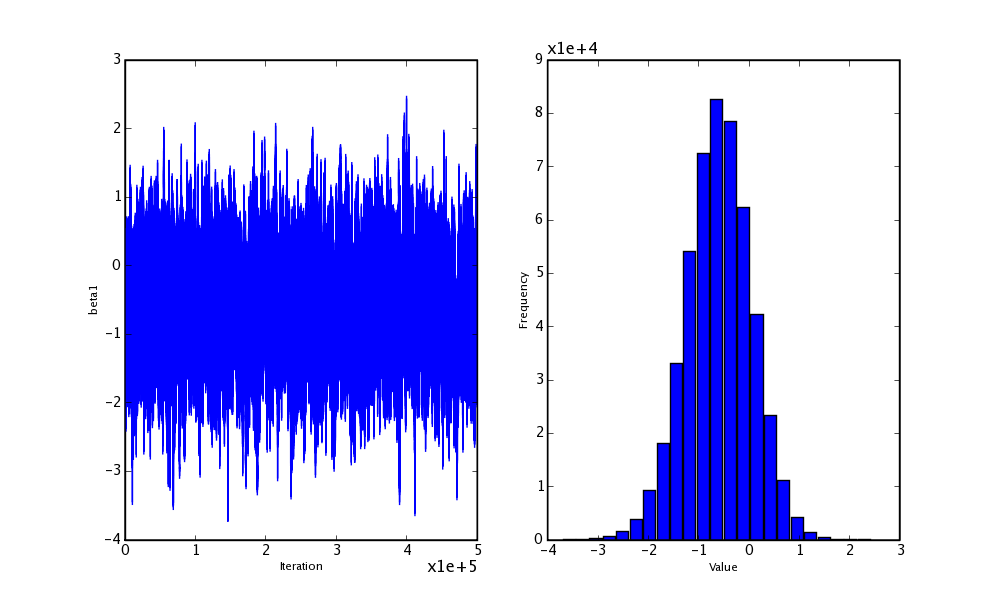
\includegraphics[scale=0.4]{sample_output.png}
    \end{center}
    \caption{Sample trace (left) and histogram (right) from Metropolis-Hastings simulation using PyMC.}
    \label{fig:sample_output}
\end{figure}

Valid inference relies on the assumption that sample values are random (but not necessarily independent) draws from the limiting distribution of the Markov chain. Typically, since unknown parameters are initialized arbitrarily, it is unlikely that the entire sample satisfies this assumption. It is usual, therefore, to discard the first portion of the sample, up to some specified proportion. The appropriate size of this ``burn-in" period is usually determined  \emph{a priori}, sometimes with the assistance of a variety of convergence diagnostics (discussed later). The number of iterations required for convergence varies strongly with the nature of the target posterior distribution and the efficiency of the chosen MCMC algorithm.

Since the sample is derived from a Markov chain, it is necessarily autocorrelated. Poorly-mixing simulations will exhibit autocorrelation more acutely, as successive samples will be relatively close (in parameter space) to their predecessors. Therefore, it is often desirable to ``thin" the sample output, by retaining every $k$ sample from the chain, where $k$ is determined by the severity of the autocorrelation function.


\section{The \texttt{SamplingMethod} class}\label{sec:SamplingMethod}
Sampling methods are responsible for making parameters or groups of parameters take single MCMC steps. PyMC provides several standard sampling methods, including \texttt{OneAtATimeMetropolis}, but \texttt{SamplingMethod} is designed to be subclassed to handle particular types of probability submodels. When writing your own sampling methods, try to make them embeddable; that is, try to make them work reliably regardless of what the probability model looks like outside of the submodel over which they have jurisdiction. If you do this, you'll accumulate a library of sampling methods that can be easily stuck together to fit new probability models, and you won't have to keep rewriting them.

\begin{figure}[hhhhhhhhh]
    \centering
    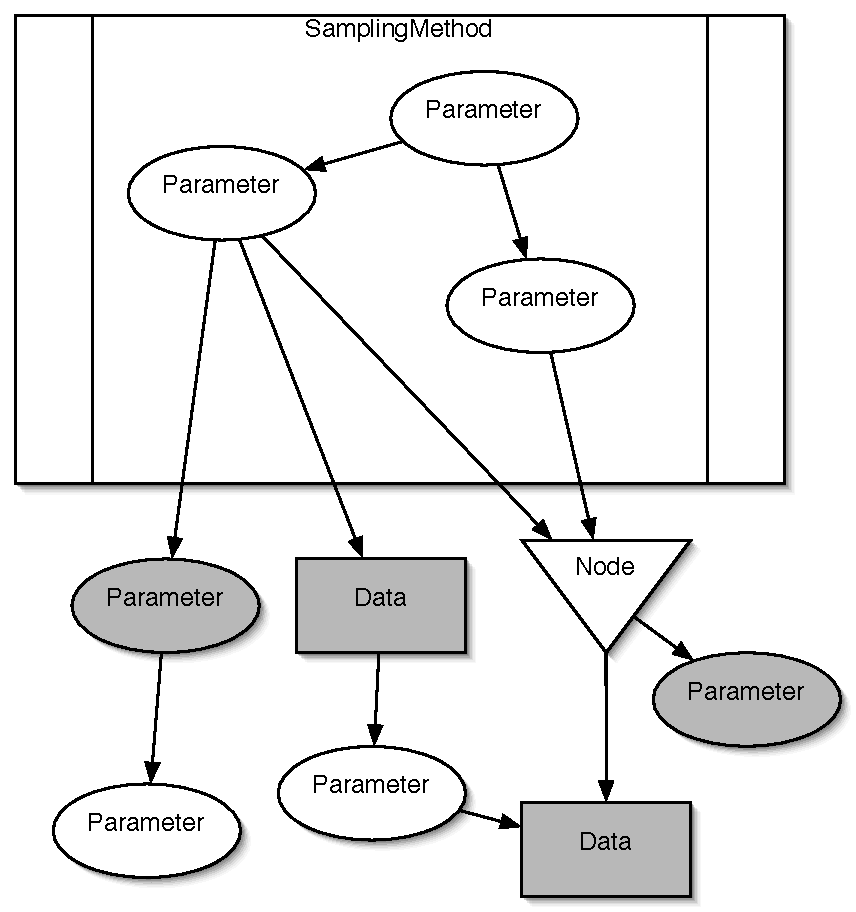
\epsfig{file=sampmethod_children.pdf,width=6cm}
    \caption{The children of a sampling method. The parameters under the sampling method's jurisdiction are shown on a plate. The children of the sampling method are the parameters (regardless of \texttt{isdata}) which depend on the sampling method's parameters either directly or via an unbroken sequence of nodes, and which aren't in the sampling method's parameters.}
    \label{fig:sampmethod_children}
\end{figure}

All sampling methods must be subclasses of \texttt{SamplingMethod}, which exposes the following attributes:
\begin{description}
    \item[\texttt{nodes}:] A set containing the nodes over which self has jurisdiction. Although sampling methods are primarily responsible for making parameters take Metropolis steps, it can be nice to assign nodes to them for organizational reasons.
    \item[\texttt{parameters}:] A set containing the parameters over which self has jurisdiction, with \texttt{isdata} set to false. Self will be responsible for making all of these parameters take single MCMC steps.
    \item[\texttt{data}:] A set containing the parameters over which self has jurisdiction, with \texttt{isdata} set to true. Again, this attribute is provided for the sake of organization.
    \item[\texttt{pymc\_objects}:] The union of \texttt{nodes}, \texttt{parameters}, and \texttt{data}.
    \item[\texttt{children}:] The union of all the nearest descendants of self's parameters that are themselves parameters, differenced with the set of self's parameters. See figure \ref{fig:sampmethod_children}.
    \item[\texttt{loglike}:] The log-probability of self's children given self's parameters' current values. The sum of self's parameters' \texttt{logp} attributes plus \texttt{self.loglike}  gives the total log joint probability of self's parameters, up to superfluous constants. This attribute will be needed by most embeddable sampling methods. Loglike is recomputed every time it's accessed.
    \item[\texttt{\_asf}]: A catchall name for tunable sampling parameters.
\end{description}

\texttt{SamplingMethod} has the following methods, which aren't implemented in the base class:
\begin{description}
    \item[\texttt{sample()}:] \texttt{Model} will call this method for each sampling method. When it is called, self must cause each of its parameters to take an MCMC step. All subclasses must implement this method.
    \item[\texttt{tune()}:] \texttt{Model} will also call this method for each sampling method, but implementation is optional. When it is called, self should tune its stepping strategy somehow, possibly by adjusting \texttt{\_asf}.
\end{description}


\subsection{\texttt{OneAtATimeMetropolis}}\label{sub:OAATM}
This is PyMC's basic sampling method. If \texttt{Model}, on instantiation, finds that a parameter is not handled by any sampling method, it will create an instance of \texttt{OneAtATimeMetropolis} to handle that parameter. The easiest way to explain this simple object is just to display its source code: \textbf{XXX replace when tune() and more \_dist's are implemented}
\begin{verbatim}
class OneAtATimeMetropolis(SamplingMethod):

    def __init__(self, parameter, scale=1, dist='Normal'):
        SamplingMethod.__init__(self,[parameter])
        self.parameter = parameter
        self.proposal_sig = ones(shape(self.parameter.value)) * \
                            abs(self.parameter.value) * scale
        self.proposal_deviate = zeros(shape(self.parameter.value),dtype=float)
        self._dist = dist

    def step(self):

        # Probability and likelihood for parameter's current value:

        logp = self.parameter.logp
        loglike = self.loglike

        # Sample a candidate value
        self.propose()

        # Probability and likelihood for parameter's proposed value:
        try:
            logp_p = self.parameter.logp

        # Reject jumps to illegal values
        except LikelihoodError:
            self.parameter.revert()
            self._rejected += 1
            return

        loglike_p = self.loglike

        # Test
        if log(random()) > logp_p + loglike_p - logp - loglike:
            # Revert parameter (reject) if fail
            self.parameter.revert()

            self._rejected += 1
        else:
            # Do nothing (accept) if pass
            self._accepted += 1

    def propose(self):

        if self._dist == 'RoundedNormal':
            self.parameter.value = round(rnormal(self.parameter.value,self.proposal_sig))
        # Default to normal random-walk proposal
        else:
            self.parameter.value = rnormal(self.parameter.value,self.proposal_sig)

    def tune(self):
        #
        # Adjust _asf according to some heuristic
        #
        pass
\end{verbatim}

Note that a proposal is made by actually updating the parameter's value, and jumps are rejected by calling the parameter's \texttt{revert()} method. This procedure lets parameters and nodes make the best use of their internal caches and minimizes the computation that needs to be done. Note also that, by convention, log-probability evaluation functions raise a \texttt{LikelihoodError} rather than returning \texttt{-inf} when the probability or density of a value is zero. This is done for compatibility with fortran 77, which does not recognize \texttt{inf}s. The function \texttt{random()}, from numpy, returns a random number uniformly distributed between 0 and 1.


\subsection{Other sampling methods provided with the distribution}\label{sub:other_sm}
\textbf{XXX} JointMetropolis, OpenCapture, ClosedCapture, whatever else.



%(end)

\section{The \texttt{Sampler} class}\label{sec:Sampler}
The Sampler class is a subclass of Model. In addition to those inherited from Model, it has the following attributes:
\begin{description}
	\item[\texttt{sampling\_methods}:]
\end{description}
and the following methods:
\begin{description}
	\item[\texttt{tune()}:]
	\item[\texttt{sample()}:]
	\item[\texttt{interactive\_sample()}:] 
\end{description}


\chapter{Diagnostics} %(fold)

\section{Convergence Diagnostics}

Valid inferences from sequences of MCMC samples are based on the assumption that the samples are derived from the true posterior distribution of interest. Theory guarantees this condition as the number of iterations approaches infinity. It is important, therefore, to determine the minimum number of samples required to ensure a reasonable approximation to the target posterior density. Unfortunately, no universal threshold exists across all problems, so convergence must be assessed independently each time MCMC estimation is performed. The procedures for verifying convergence are collectively known as convergence diagnostics.

One approach to analyzing convergence is analytical, whereby the variance of the sample at different sections of the chain are compared to that of the limiting distribution. These methods use distance metrics to analyze convergence, or place theoretical bounds on the sample variance, and though they are promising, they are generally difficult to use and are not prominent in the MCMC literature. More common is a statistical approach to assessing convergence. With this approach, rather than considering the properties of the theoretical target distribution, only the statistical properties of the observed chain are analyzed. Reliance on the sample alone restricts such convergence criteria to heuristics; that is, convergence cannot be guaranteed. Although evidence for lack of convergence using statistical convergence diagnostics will correctly imply lack of convergence in the chain, the absence of such evidence will not \emph{guarantee} convergence in the chain. Nevertheless, negative results for one or more criteria will provide some measure of assurance to most users that their sample will provide valid inferences.

For most simple models, convergence will occur quickly, sometimes within a the first several hundred iterations, after which all remaining samples of the chain may be used to calculate posterior quantities. For many more complex models, convergence requires a significantly longer burn-in period; sometimes  orders of magnitude more samples are needed. Frequently, lack of convergence will be caused by poor mixing (Figure \ref{fig:mix}). Recall that \emph{mixing} refers to the degree to which the Markov chain explores the support of the posterior distribution. Poor mixing may stem from inappropriate proposals (if one is using the Metropolis-Hastings sampler) or from attempting to estimate models with highly correlated parameters.

\begin{figure}[ht]
\begin{center}
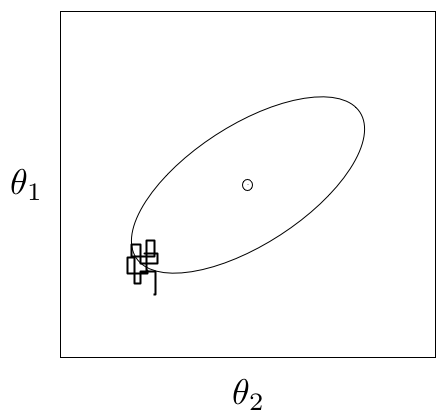
\includegraphics[height=3in]{poor_mixing.png}
\caption{An example of a poorly-mixing sample in two dimensions. Notice that the chain is trapped in a region of low probability relative to the mean (dot) and variance (oval) of the true posterior quantity.}
\label{fig:mix}
\end{center}
\end{figure}

\section*{Informal Methods}

The most straightforward approach for assessing convergence is based on simply plotting and inspecting traces and histograms of the observed MCMC sample. If the trace of values for each of the parameters exhibits asymptotic behaviour\footnote{Asymptotic behaviour implies that the variance and the mean value of the sample stays relatively constant over some arbitrary period.} over the last $m$ iterations, this may be satisfactory evidence for convergence. A similar approach involves plotting a histogram for every set of $k$ iterations (perhaps 50-100) beyond some burn in threshold $n$; if the histograms are not visibly different among the sample intervals, this is reasonable evidence for convergence. Note that such diagnostics should be carried out for each parameter estimated by the MCMC algorithm, because convergent behaviour by one parameter does not imply evidence for convergence for other parameters in the analysis. An extension of this approach can me taken when multiple parallel chains are run, rather than just a single, long chain. In this case, the final values of $c$ chains run for $n$ iterations are plotted in a histogram; just as above, this is repeated every $k$ iterations thereafter, and the histograms of the endpoints are plotted again and compared to the previous histogram. This is repeated until consecutive histograms are indistinguishable.

\begin{figure}[h]
\begin{center}
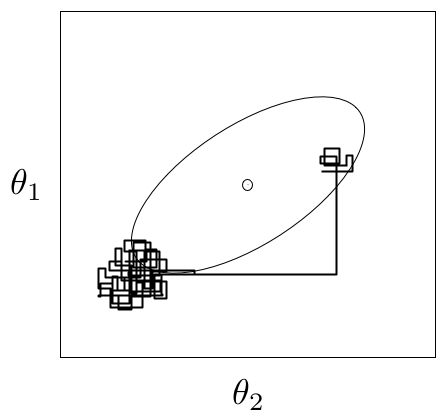
\includegraphics[height=3in]{metastable.png}
\caption{An example of metastability in a two-dimensional parameter space. The chain appears to be stable in one region of the parameter space for an extended period, then unpredictably jumps to another region of the space.}
\label{fig:metas}
\end{center}
\end{figure}

Another \emph{ad hoc} method for detecting convergence is to examine the traces of several MCMC chains initialized with different starting values. Overlaying these traces on the same set of axes should (if convergence has occurred) show each chain tending toward the same equilibrium value, with approximately the same variance. Recall that the tendency for some Markov chains to converge to the true (unknown) value from diverse initial values is called \emph{ergodicity}. This property is guaranteed by the reversible chains constructed using MCMC, and should be observable using this technique. Again, however, this approach is only a heuristic method, and cannot always detect lack of convergence, even though chains may appear ergodic.

A principle reason that evidence from informal techniques cannot guarantee convergence is a phenomenon called metastability. Chains may appear to have converged to the true equilibrium value, displaying excellent qualities by any of the methods described above. However, after some period of stability around this value, the chain may suddenly move to another region of the parameter space (Figure \ref{fig:metas}). This period of metastability can sometimes be very long, and therefore escape detection by these convergence diagnostics. Unfortunately, there is no statistical technique available for detecting metastability.

\section*{Formal Methods}

Along with the \emph{ad hoc} techniques described above, a number of more formal methods exist which are prevalent in the literature. These are considered more formal because they are based on existing statistical methods, such as time series analysis.

PyMC includes one formal convergence diagnostic method, first proposed by \citet{Geweke:1992gm}. This is a time-series approach, which compares the mean and variance of segments from the beginning and end of a single chain.
\begin{equation}
z = \frac{\bar{\theta}_a - \bar{\theta}_b}{\sqrt{Var(\theta_a) + Var(\theta_b)}}
\end{equation}
where $a$ is the early interval and $b$ the late interval. If the z-scores of these two segments are similar, it can provide evidence for convergence. PyMC plots the z-scores of the difference between various initial segments along the chain, and the last 50\% of the remaining chain. If the chain has converged, the majority of points should fall within 2 standard deviations of zero. Calling the convergence method results in a diagnostic plot for each model parameter.

\subsubsection{Method Usage}
\begin{verbatim}
sampler.convergence(first=0.1, last=0.5, intervals=20, burn=0, thin=1, chain=-1, plot=True)
\end{verbatim}
\begin{itemize}

\item \verb=first= (optional): First portion of chain to be used in Geweke diagnostic. Defaults to 0.1 (i.e. first 10% of chain).

\item \verb=last= (optional): Last portion of chain to be used in Geweke diagnostic. Defaults to 0.5 (i.e. last 50% of chain).

\item \verb=intervals= (optional): Number of sub-chains to analyze. Defaults to 20.

\item \verb=burn (optional)=: Number of burn-in iterations to exclude. Defaults to 0 (\emph{i.e.} no burn-in).

\item \verb=thin (optional)=: Thinning factor. Defaults to 1 (\emph{i.e.} no thinning).

\item \verb=chain= (optional): Chain to be analyzed. Defaults to -1 (\emph{i.e}. last chain).

\item \verb=plot= (optional): Plotting flag. Defaults to True.
\end{itemize}
Comprehensive convergence diagnostics are available in the \href{http://lib.stat.cmu.edu/R/CRAN/}{R statistical package}, via the \href{http://www-fis.iarc.fr/coda/}{CODA module}. The \verb=MetropolisHastings= class in PyMC includes a method for exporting model traces in a format that may be directly read by CODA.

\subsubsection{Method Usage}
\begin{verbatim}
sampler.coda_output(filename="coda", burn=0, thin=1)
\end{verbatim}
\begin{itemize}

\item \verb=filename= (optional): Filename of coda output files. Defaults to ``coda''.

\item \verb=burn (optional)=: Number of burn-in iterations to exclude. Defaults to 0 (\emph{i.e.} no burn-in).

\item \verb=thin (optional)=: Thinning factor. Defaults to 1 (\emph{i.e.} no thinning).

\end{itemize}
Calling \verb=coda_output= yields a \verb=.out= file containing raw trace values and a \verb=.ind= file containing indices.

\section{Goodness-of-Fit}

PyMC provides a flexible method for assessing goodness-of-fit (GOF) of models following MCMC estimation. Following \citet{Gelman:1996gp}, the \verb=goodness= method from the \verb=MetropolisHastings= sampler assesses GOF using a simple discrepancy measure for each component of the likelihood. This measure compares the deviance of the data from the expected parameter values to deviance of simulated data from the expected parameter values. Data are simulated based on samples from the trace of all the parameters. These observed and simulated deviances are plotted against one another to yield GOF plots:

Evidence for lack of fit is apparent when points do not fall on either side of the diagonal in approximately the same numbers; the example above shows very good fit. One plot is generated for every component of the likelihood bearing the same name. Additionally, PyMC reports a GOF statistic (which some authors regrettably call the Bayesian $p$-value), which is simply the proportion of points where the simulated deviance is greater than the observed deviance. This value should be close to 0.5 for a well-fit model.

\subsubsection{Method Usage}
\begin{verbatim}
sampler.goodness(iterations, plot=True, loss='squared', burn=0, thin=1, chain=-1, composite=False)
\end{verbatim}

\begin{itemize}

\item \verb=iterations=: Number of GOF iterations to run.

\item \verb=plot (optional)=: Plotting flag. Defaults to True.

\item \verb=loss (optional)=: Loss function to use. Valid arguments include ‘squared’, ‘absolute’ and ‘chi-square’. Defaults to ‘squared’.

\item \verb=burn (optional)=: Number of burn-in iterations to exclude. Defaults to 0 (\emph{i.e.} no burn-in).

\item \verb=thin (optional)=: Thinning factor. Defaults to 1 (\emph{i.e.} no thinning).

\item \verb=chain (optional)=: Chain to be analyzed. Defaults to -1 (\emph{i.e.} last chain).

\item \verb=composite (optional)=: Flag for composite GOF analysis (\emph{i.e.} based on all chains combined). Defaults to False.
\end{itemize}


\subsubsection{Method Usage}
\section{Autocorrelation Plots}

Samples from MCMC algorithms are ususally autocorrelated, due partly to the inherent Markovian dependence structure. The degree of autocorrelation can be quantified using the autocorrelation function:
\begin{eqnarray*}
    \rho_k &=& \frac{\mbox{Cov}(X_t, X_{t+k})}{\sqrt{\mbox{Var}(X_t)\mbox{Var}(X_{t+k})}} \\
            &=& \frac{E[(X_t - \theta)(X_{t+k} - \theta)]}{\sqrt{E[(X_t - \theta)^2] E[(X_{t+k} - \theta)^2]}}
\end{eqnarray*}
The \verb=MetropolisHastings= class includes a method for plotting the autocorrelation function for each parameter in the sampler (Figure \ref{fig:autocorr}). This allows users to examine the relationship among successive samples within sampled chains. Significant autocorrelation suggests that chains require thinning prior to use of the posterior statistics for inference.

\begin{figure}[htbp]
        \begin{center}
        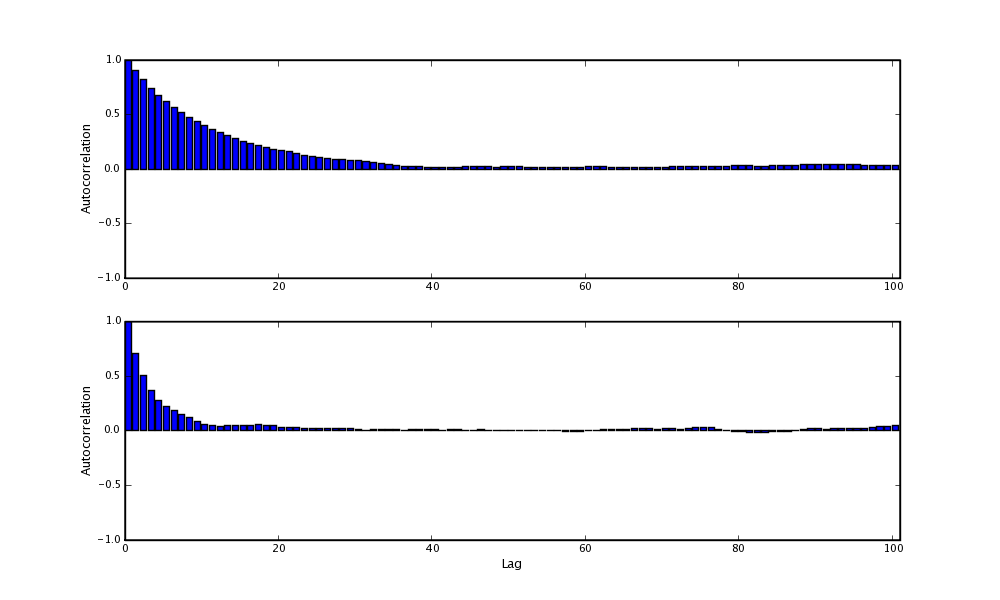
\includegraphics[scale=0.4]{autocorr.png}
    \end{center}
    \caption{Sample autocorrelation plots for two Poisson parameters from coal mining disasters example model.}
    \label{fig:autocorr}
\end{figure}

\begin{verbatim}
sampler.autocorrelation(max_lag=100, burn=0, thin=1, chain=-1)
\end{verbatim}

\begin{itemize}

\item \verb=max_lag (optional)=: Maximum time lag to calculate autocorrelation. Defaults to 100 iterations.

\item \verb=burn (optional)=: Number of burn-in iterations to exclude. Defaults to 0 (\emph{i.e.} no burn-in).

\item \verb=thin (optional)=: Thinning factor. Defaults to 1 (\emph{i.e.} no thinning).

\item \verb=chain (optional)=: Chain to be analyzed. Defaults to -1 (\emph{i.e}. last chain).
\end{itemize}

%(end)

\chapter{Advanced topics}

\section{How to make PyMC run as fast as possible}\label{sec:fast} % (fold)
\subsection{Profile your code}\label{sub:profile_your_code} % (fold)
So you can see where the bottlenecks are. It's easy in IPython. Timing your code is helpful too.

\subsection{Write fast log-probability functions}\label{sub:write_fast_log_probability_functions} % (fold)

PyMC aims to provide a fast and user-friendly interface to several standard probability distributions. However, we're not able to anticipate every usage case. We're not even going to try, but you can provide any Python-callable function you want. This is often fruitful, because in most cases the easiest way to buy efficiency is to optimize log-probability functions. Try Weave or f2py. Consider the DisasterSampler example with custom log-probability functions- speeds up by a factor of three! We've tried to keep the overhead low so optimization is worth your while. Quick runthrough of f2py.
\subsection{Optimize custom subsamplers}\label{sub:optimize_custom_subsamplers}
The second-most-likely place for a bottleneck is in a custom SubSampler. Model itself is probably not the bottleneck. Weave and f2py might be helpful here, too.

\bibliographystyle{plainnat}
\bibliography{pymc}


\appendix

\chapter{Probability distributions}
David
Link to the epydoc generated API ?
\chapter{epydoc class reference?}

\chapter{Database backends}
David
Link to the epydoc generated API ?

\end{document}
 